\normaltrue
\correctiontrue

%\UPSTIidClasse{11} % 11 sup, 12 spé
%\newcommand{\UPSTIidClasse}{12}

\exer{Mouvement TR  $\star$ \label{CIN:02:B2:13:06:02}}
\setcounter{question}{0}\marginnote{\UPSTIcompetence{B2-13}}
\index{Compétence B2-13}\index{Compétence CIN-02}
\index{Mécanisme à 1 translation et 1 rotation}
\ifcorrection
\else
\marginnote{\textbf{Pas de corrigé pour cet exercice.}}
\fi

\ifprof
\else
Soit le mécanisme suivant. On a $\vect{AB}=\lambda(t)\vect{i_0}$ et $\vect{BC}=R\vect{i_2}$ avec $R=\SI{30}{mm}$. 
\begin{marginfigure}
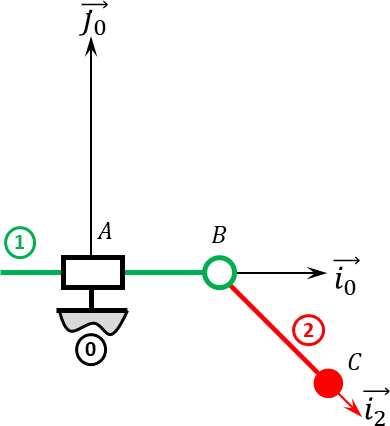
\includegraphics[width=\linewidth]{06_TR_01a}
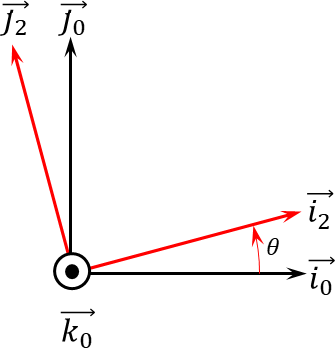
\includegraphics[width=\linewidth]{06_TR_01b}
\end{marginfigure}
\fi

% ================================
\ifprof
\else
\ifcolle
\else
\marginnote{\begin{solution}
\begin{enumerate}
\item $\vectv{C}{2}{0} =\dot{\lambda}(t) \vect{i_0} + R \dot{\theta} \vj{2}$.
\item $\torseurcin{V}{2}{0}=\torseurl{\vecto{2}{0}=\dot{\theta}\vk{0}}{\vectv{C}{2}{0}}{C}$.
\item $\vectg{C}{2}{0} =\ddot{\lambda}(t) \vect{i_0} + R \left(\ddot{\theta} \vj{2} - \dot{\theta}^2 \vi{2}\right) $.
\end{enumerate} 
\end{solution}}
\fi
\marginnote{Corrigé  voir \ref{CIN:02:B2:13:06:02}.}
\fi
% ================================

\question{Déterminer $\vectv{C}{2}{0}$ par dérivation vectorielle ou par composition.}
\ifprof ~\\

\textbf{Méthode 1 -- Dérivation vectorielle} ~\\

$\vectv{C}{2}{0} =$
$\deriv{\vect{AC}}{\rep{0}}= \deriv{\vect{AB}}{\rep{0}}+\deriv{\vect{BC}}{\rep{0}}$
$= \dot{\lambda}(t) \vect{i_0} + R \deriv{\vi{2}}{\rep{0}}$
$= \dot{\lambda}(t) \vect{i_0} + R \dot{\theta} \vj{2}$
%$= \ddot{\lambda}(t) \vect{i_0} + R \left(\ddot{\theta} \vj{2} - \dot{\theta}^2 \vi{2}\right) $.

\textbf{Méthode 2 -- Composition du torseur cinématique} ~\\
$\vectv{C}{2}{0} =\vectv{C}{2}{1} +\vectv{C}{1}{0} $

Pour tout point $P$, $\vectv{P}{1}{0}=\dot{\lambda}\vi{0}$.

$\babarv{C}{B}{2}{1}=-R\vi{2}\wedge \dot{\theta}\vk{0}=R\dot{\theta}\vj{2}$.

On a donc $\vectv{C}{2}{0}=\dot{\lambda}\vi{0}+R\dot{\theta}\vj{2}$.

\else
\fi

\question{Donner le torseur cinématique $\torseurcin{V}{2}{0}$ au point $C$.}
\ifprof

$\torseurcin{V}{2}{0}=\torseurl{\vecto{2}{0}=\dot{\theta}\vk{0}}{\vectv{C}{2}{0}=\dot{\lambda}\vi{0}+R\dot{\theta}\vj{2}}{C}$.


\else
\fi

\question{Déterminer $\vectg{C}{2}{0}$.}
\ifprof ~\\

$\vectg{C}{2}{0} =\deriv{\vectv{C}{2}{0}}{\rep{0}}$
$= \ddot{\lambda}(t) \vect{i_0} + R \deriv{\dot{\theta} \vj{2}}{\rep0}$
$= \ddot{\lambda}(t) \vect{i_0} + R \left(\ddot{\theta} \vj{2} - \dot{\theta}^2 \vi{2}\right) $.
\else
\fi

